\documentclass[]{spie}  %>>> use for US letter paper
%\documentclass[a4paper]{spie}  %>>> use this instead for A4 paper
%\documentclass[nocompress]{spie}  %>>> to avoid compression of citations

\renewcommand{\baselinestretch}{1.0} % Change to 1.65 for double spacing
 
\usepackage{amsmath,amsfonts,amssymb}
\usepackage{graphicx}
\usepackage[colorlinks=true, allcolors=blue]{hyperref}
\usepackage{glossaries}
\title{Simulating the Effects of Exozodiacal Dust in WFIRST CGI observations}

\author[a]{Ewan S. Douglas}
\author[b]{John Debes}
\author[a]{Kian Miliani}
\affil[a]{University of Arizona, Tucson, AZ, USA}
\affil[b]{STScI, Baltimore, MD, USA}

\authorinfo{Further author information: (Send correspondence to A.A.A.)\\A.A.A.: E-mail: aaa@tbk2.edu, Telephone: 1 505 123 1234\\  B.B.A.: E-mail: bba@cmp.com, Telephone: +33 (0)1 98 76 54 32}

% Option to view page numbers
\pagestyle{empty} % change to \pagestyle{plain} for page numbers   
\setcounter{page}{301} % Set start page numbering at e.g. 301
 
\begin{document} 
\maketitle

\begin{abstract}

\end{abstract}
% astronomical and space physics acronyms for use with LaTeX glossaries package.

%to copy without git, try: 
% wget https://gist.githubusercontent.com/douglase/78b39cfa4501f0ce43fe/raw//acronyms.tex
% or if you want to overwrite:
% curl -O https://gist.githubusercontent.com/douglase/78b39cfa4501f0ce43fe/raw//acronyms.tex

%units
\newacronym{AU}{AU}{astronomical Unit [1.5e11 m]}  
\newacronym{pc}{pc}{parsec}
\newacronym{mas}{mas}{milliarcsecond}
\newacronym{nm}{nm}{nanometer}
\newacronym{CTE}{CTE}{coefficient of thermal expansion}

%objects
\newacronym{smc}{SMC}{Small Magellanic Cloud}
\newacronym{lmc}{LMC}{Large Magellanic Cloud}
\newacronym{ism}{ISM}{interstellar medium}
\newacronym{mw}{MW}{Milky Way}
\newacronym{epseri}{$\epsilon$ Eri}{Epsilon Eridani}
\newacronym{EKB}{EKB}{Edgeworth-Kuiper Belt}


%radiative transfer
\newacronym{CFR}{CFR}{Complete Frequency Redistribution}

%organizations
\newacronym{nasa}{NASA}{National Aeronautics and Space Agency}
\newacronym{esa}{ESA}{European Space Agency}
\newacronym{omi}{OMI}{\textit{Optical Mechanics Inc.}}
\newacronym{gsfc}{GSFC}{\gls{nasa} Goddard Space Flight Center}
\newacronym{stsci}{STScI}{Space Telescope Science Institute}
\newacronym{nsroc}{NSROC}{\gls{nasa} Sounding Rocket Operations Contract}
\newacronym{wff}{WFF}{\gls{nasa} Wallops Flight Facility}
\newacronym{wsmr}{WSMR}{White Sands Missile Range}

%technologies and sensors
\newacronym{irac}{IRAC}{Infrared Array Camera}
\newacronym[plural=CCDs, firstplural=charge-coupled devices (CCDs)]{ccd}{CCD}{charge-coupled device}
\newacronym[plural=EMCCDs, firstplural=electron multiplying charge-coupled devices (EMCCDs)]{EMCCD}{EMCCD}{electron multiplying charge-coupled device}

\newacronym{DM}{DM}{Deformable Mirror}
\newacronym{MCP}{MCP}{ Microchannel Plate }
\newacronym{ipc}{IPC}{Image Proportional Counter}
\newacronym{cots}{COTS}{Commercial Off-The-Shelf}
\newacronym{ISR}{ISR}{Incoherent Scatter Radar }
\newacronym{atcamera}{AT}{Angle Tracker}
\newacronym{MEMS}{MEMS}{microelectromechanical systems}
\newacronym{QE}{QE}{quantum efficiency}
\newacronym{RTD}{RTD}{Resistance Temperature Detector}
\newacronym{PID}{PID}{Proportional-Integral-Derivative}
\newacronym{PRNU}{PRNU}{photo response non-uniformity}
\newacronym{DSNU}{PRNU}{dark signal non-uniformity}
\newacronym{CMOS}{CMOS}{complementary metal–oxide–semiconductor}
\newacronym{TRL}{TRL}{technology readiness level}

%optics
\newacronym{FOV}{FOV}{field-of-view}
\newacronym{NIR}{NIR}{near-infrared}
\newacronym{PV}{PV}{Peak-to-Valley}
\newacronym{MRF}{MRF}{Magnetorheological finishing}
\newacronym{AO}{AO}{Adaptive Optics}
\newacronym{TTP}{TTP}{tip, tilt, and piston}
\newacronym{FPS}{FPS}{fine pointing system}
\newacronym{SHWFS}{SHWFS}{Shack-Hartmann Wavefront Sensor}
\newacronym{OAP}{OAP}{off-axis parabola}
\newacronym{LGS}{LGS}{laser guide star}
\newacronym{WFCS}{WFCS}{wavefront control system}
\newacronym{OPD}{OPD}{optical path difference}

%%sounding Rockets:
\newacronym{acs}{ACS}{Attitude Control System}
\newacronym{orsa}{ORSA}{Ogive Recovery System Assembly}
\newacronym{gse}{GSE}{Ground Station Equipment}
\newacronym{FSM}{FSM}{Fast Steering Mirror}


%%high contrast imaging:
\newacronym{WFS}{WFS}{wavefront sensor}
\newacronym{LSI}{LSI}{Lateral Shearing Interferometer}
\newacronym{VVC}{VVC}{Vector Vortex Coronagraph}
\newacronym{VNC}{VNC}{Visible Nulling Coronagraph}
\newacronym{CGI}{CGI}{Coronagraph Instrument}
\newacronym{IWA}{IWA}{Inner Working Angle}
\newacronym{OWA}{OWA}{Outer Working Angle}
\newacronym{NPZT}{N-PZT}{Nuller piezoelectric transducer}
\newacronym{ZWFS}{ZWFS}{Zernike wavefront sensor}
\newacronym{SPC}{SPC}{Shaped Pupil Coronagraph}
\newacronym{HLC}{HLC}{Hybrid-Lyot Coronagraph}
\newacronym{ADI}{ADI}{angular differential imaging}
\newacronym{RDI}{RDI}{reference differential imaging}

%observatories and instruments
\newacronym{HST}{HST}{Hubble Space Telescope}
\newacronym{GPS}{GPS}{Global Positioning System}
\newacronym{ISS}{ISS}{International Space Station}
\newacronym[description=Advanced CCD Imaging Spectrometer]{acis}{ACIS}{Advanced \gls{ccd} Imaging Spectrometer}
\newacronym{stis}{STIS}{\textit{Space Telescope Imaging Spectrograph}}
\newacronym{mcp}{MCP}{Microchannel Plate}
\newacronym{jwst}{JWST}{$\textit{James Webb Space Telescope}$}
\newacronym{fuse}{FUSE}{$\textit{FUSE}$}
\newacronym{galex}{GALEX}{$\textit{Galaxy Evolution Explorer}$}
\newacronym{spitzer}{Spitzer}{$\textit{Spitzer Space Telescope}$}
\newacronym{mips}{MIPS}{Multiband Imaging Photometer for \gls{spitzer}}
\newacronym{gissmo}{GISSMO}{Gas Ionization Solar Spectral Monitor}
\newacronym{iue}{IUE}{International Ultraviolet Explorer}
\newacronym{spinr}{SPINR}{$\textit{Spectrograph for Photometric Imaging with Numeric Reconstruction}$}
\newacronym{imager}{IMAGER}{$\textit{Interstellar Medium Absorption Gradient Experiment Rocket}$}
\newacronym{TPF-C}{TPF-C}{Terrestrial Planet Finder Coronagraph}
\newacronym{RAIDS}{RAIDS}{Atmospheric and Ionospheric Detection System }
\newacronym{mama}{MAMA}{Multi-Anode Microchannel Array}
\newacronym{ATLAST}{ATLAST}{Advanced Technology Large Aperture Space Telescope}
\newacronym{PICTURE}{PICTURE}{Planet Imaging Concept Testbed Using a Rocket Experiment}
\newacronym{LITES}{LITES}{Limb-imaging Ionospheric and Thermospheric
Extreme-ultraviolet Spectrograph}
\newacronym{LBT}{LBT}{Large Binocular Telescope}
\newacronym{LBTI}{LBTI}{Large Binocular Telescope Interferometer}
\newacronym{KIN}{KIN}{Keck Interferometer Nuller}
\newacronym{SHARPI}{SHARPI}{Solar High-Angular Resolution Photometric Imager}
\newacronym{IRAS}{IRAS}{Infrared Astronomical Satellite}
\newacronym{HARPS}{HARPS}{High Accuracy Radial velocity Planetary}
\newacronym{hstSTIS}{STIS}{Space Telescope Imaging Spectrograph}
\newacronym{spitzerIRAC}{IRAC}{Infrared Array Camera}
\newacronym{spitzerMIPS}{MIPS}{Multiband Imaging Photometer for Spitzer}
\newacronym{spitzerIRS}{IRS}{Infrared Spectrograph}
\newacronym{CHARA}{CHARA}{Center for High Angular Resolution Astronomy}
\newacronym{wfirst-afta}{WFIRST-AFTA}{Wide-Field InfrarRed Survey
Telescope-Astrophysics Focused Telescope Assets}
\newacronym{GPI}{GPI}{Gemini Planet Imager}
\newacronym{WFIRST}{WFIRST}{Wide-Field InfrarRed Survey Telescope}
\newacronym{HabEx}{HabEx}{Habitable Exoplanet Observatory Mission Concept}
\newacronym{LUVOIR}{LUVOIR}{Large UV/Optical/Infrared Surveyor}
\newacronym{FGS}{FGS}{Fine Guidance Sensor}
\newacronym{STIS}{STIS}{Space Telescope Imaging Spectrograph}
\newacronym{MGHPCC}{MGHPCC}{Massachusetts Green High Performance
Computing Center}
\newacronym{WISE}{WISE}{Wide-field Infrared Survey Explorer}
\newacronym{ALMA}{ALMA}{Atacama Large Millimeter Array}
\newacronym{GRAIL}{GRAIL}{Gravity Recovery and Interior Laboratory}

%software
\newacronym{AURIC}{AURIC}{The Atmospheric Ultraviolet Radiance Integrated Code} 
\newacronym{FFT}{FFT}{Fast Fourier Transform  }
\newacronym{MODTRAN}{MODTRAN   }{ MODerate resolution atmospheric TRANsmission }
\newacronym{idl}{IDL}{$\textit {Interactive Data Language}$}
\newacronym[sort=NED,description=NASA/IPAC Extragalactic Database]{ned}{NED}{\gls{nasa}/\gls{ipac} Extragalactic Database}
\newacronym{iraf}{IRAF}{Image Reduction and Analysis Facility}
\newacronym{wcs}{WCS}{World Coordinate System}
\newacronym{pegase}{PEGASE}{$\textit{Projet d'Etude des GAlaxies par Synthese Evolutive}$}
\newacronym{dirty}{DIRTY}{$\textit{DustI Radiative Transfer, Yeah!}$}
\newacronym{CUDA}{CUDA}{Compute Unified Device Architecture}
\newacronym{KLIP}{KLIP}{Karhunen-Lo`eve Image Processing}

%earth's atmosphere and ionosphere:
\newacronym{MSIS}{MSIS}{Mass Spectrometer Incoherent Scatter Radar}
\newacronym{nmf2}{$N_m$}{F2-Region Peak density}
\newacronym{hmf2}{$h_m$}{F2-Region Peak height}
\newacronym{H}{$H$}{F2-Region Scale Height}

%misc jargon
\newacronym{isr}{ISR}{Incoherent Scatter Radar}
\newacronym[description=TLA Within Another Acronym]{twaa}{TWAA}{\gls{tla} Within Another Acronym}
\newacronym[plural=SNe, firstplural=Supernovae (SNe)]{sn}{SN}{Supernova}
\newacronym{EUV}{EUV}{Extreme-Ultraviolet }
\newacronym{EUVS}{EUVS}{\gls{EUV} Spectrograph}
\newacronym{F2}{F2}{Ionospheric Chapman F Layer }
\newacronym{F10.7}{F10.7}{ 10.7 cm radio flux [10$^{-22}$ W m$^{-2}$ Hz$^{-1}$]  }
\newacronym{FUV}{FUV}{far-ultraviolet }
\newacronym{IR}{IR}{infrared}
\newacronym{MUV}{MUV}{mid-ultraviolet }
\newacronym{NUV}{NUV}{near-ultraviolet }
\newacronym{O$^+$}{O$^+$}{Singly Ionized Oxygen  Atom }
\newacronym{OI}{OI}{Neutral Atomic Oxygen Spectroscopic State }
\newacronym{OII}{OII}{Singly Ionized Atomic Oxygen Spectroscopic State }
\newacronym{PSF}{PSF}{point spread function}
\newacronym{$R_E$}{$R_E$}{Earth radii [$\approx$ 6400 km]  }
\newacronym{RV}{RV}{radial velocity}
\newacronym{UV}{UV}{ultraviolet }
\newacronym{WFE}{WFE}{wavefront error}
\newacronym{sed}{SED}{spectral energy distribution}
\newacronym{nir}{NIR}{near-infrared}
\newacronym{mir}{MIR}{mid-infrared}
\newacronym{ir}{IR}{infrared}
\newacronym{uv}{UV}{ultraviolet}
\newacronym[plural=PAHs, firstplural=Polycyclic Aromatic Hydrocarbons (PAHs)]{pah}{PAH}{Polycyclic Aromatic Hydrocarbon}
\newacronym{obsid}{OBSID}{Observation Identification}
\newacronym{SZA}{SZA}{Solar Zenith Angle}
\newacronym{TLE}{TLE}{Two Line Element set}
\newacronym{DOF}{DOF}{degrees-of-freedom}
\newacronym{PZT}{PZT}{lead zirconate titanate}
\newacronym{ADCS}{ADCS}{attitude determination and control system}
\newacronym{COTS}{COTS}{commercial off-the-shelf}
\newacronym{CDH}{C$\&$DH}{command and data handling}
\newacronym{EPS}{EPS}{electrical power system}

%stats
\newacronym{PCA}{PCA}{principal component analysis}
\newacronym{fwhm}{FWHM}{full-width-half maximum}
\newacronym{RMS}{RMS}{root mean squared}
\newacronym{RMSE}{RMSE}{root mean squared error}
\newacronym{MCMC}{MCMC}{Marcov chain Monte Carlo}
\newacronym{DIT}{DIT}{discrete inverse theory}
\newacronym{SNR}{SNR}{signal-to-noise ratio}
\newacronym{PSD}{PSD}{power spectral density}
\newacronym{NMF}{NMF}{non-negative matrix factorization}

% Include a list of keywords after the abstract 
\keywords{Manuscript format, template, SPIE Proceedings, LaTeX}

\section{INTRODUCTION}
The \gls{WFIRST} \gls{CGI} will image circumstellar environments, imaging circumstellar disks\cite{schneider}

\label{sec:intro}  % \label{} allows reference to this section
Exozodiacal dust presents 
\begin{figure}[htbp]
    \centering
    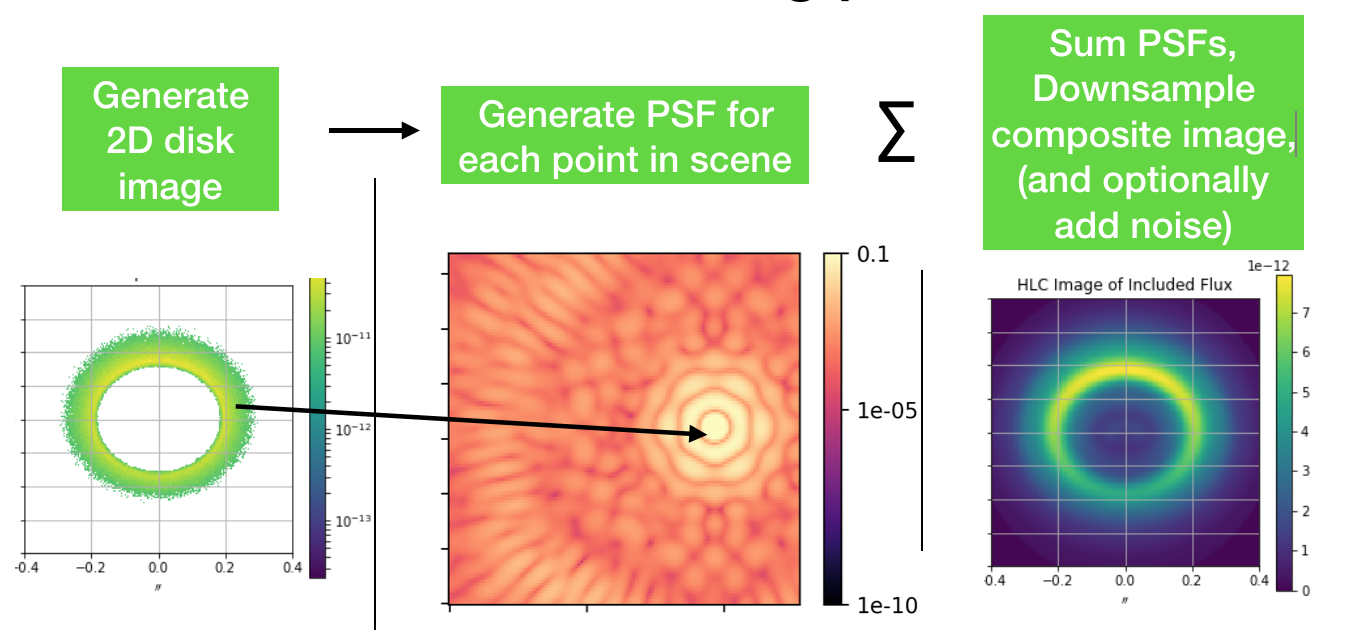
\includegraphics[width=0.95\textwidth]{flow.png}
    \caption{Simulation flow for field dependant PSF simulations of debris disks.}
    \label{fig:my_label}
\end{figure}


\begin{figure}[htbp]
    \centering
    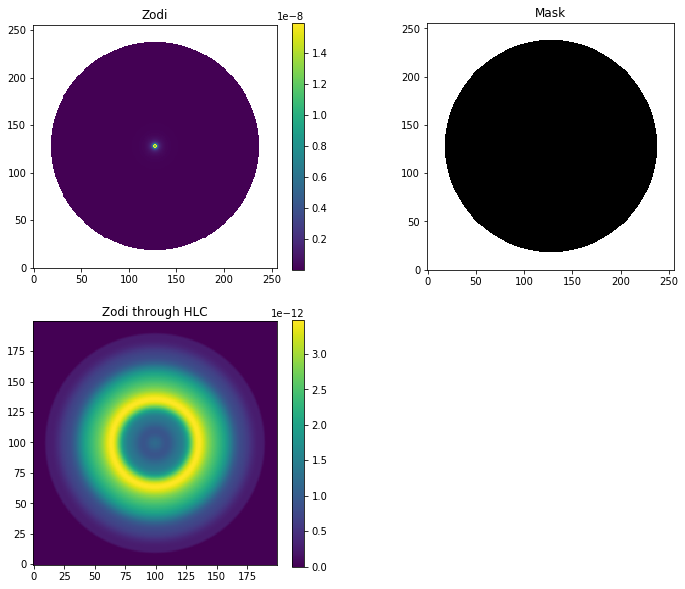
\includegraphics[width=0.95\textwidth]{Unknown-7.png}
    \caption{Simulation flow for field dependant PSF simulations of debris disks.}
    \label{fig:my_label}
    \end{figure}

    \begin{figure}[htbp]
    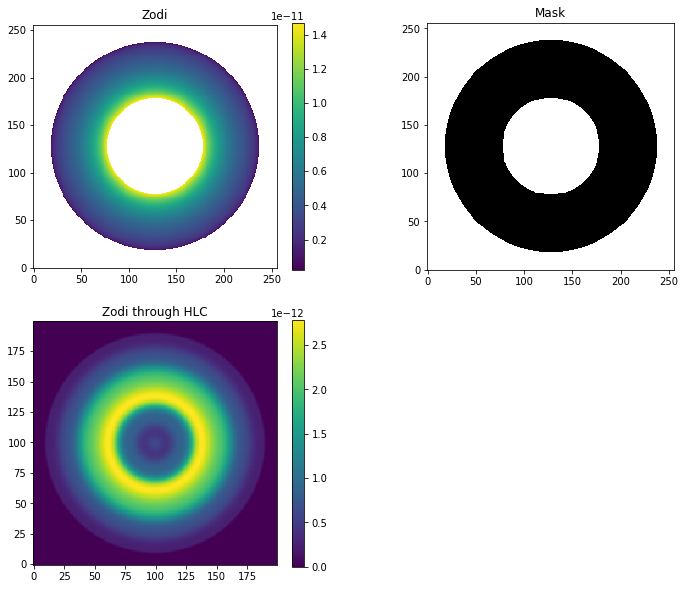
\includegraphics[width=0.95\textwidth]{Unknown-4.png}
    \caption{Simulation flow for field dependant PSF simulations of debris disks.}
    \label{fig:my_label}
\end{figure}
\section{Methods}



\section{Preliminary Results}

    
\acknowledgments % equivalent to \section*{ACKNOWLEDGMENTS}   
The authors acknowledge valuable inputs from  Vanessa Bailey,  Brian Kern, John Krist, Hanying Zhou,   and the rest of the JPL CGI team.
 Support for this work was provided by the WFIRST Science Investigation team prime award \#NNG16PJ24C.
This work was also supported by the Arizona Board of Regents Technology Research
Initiative Fund (TRIF).
This research made use of the \gls{MGHPCC} via MIT Research Computing and High Performance Computing (HPC) resources supported by the University of Arizona (UA) TRIF, UITS, and RDI and maintained by the UA Research Technologies department.

% References
%\bibliography{report} % bibliography data in report.bib
\bibliographystyle{spiebib} % makes bibtex use spiebib.bst

\end{document} 
